% backtracking worksheet template
\documentclass[leqno, 12pt]{article}
\usepackage{tikz}  
\usetikzlibrary{positioning}
\usetikzlibrary {arrows.meta}
\usepackage[a4paper, portrait, margin=1cm]{geometry}
\usepackage{multicol}
\usepackage{fancyhdr}

\tikzset{backtrack/.style={rectangle,draw=black,fill=white,
inner sep=2pt,minimum height=32pt, minimum width=20mm}}
\tikzset{backtrackeq/.style={rectangle,draw=black,fill=white,
inner sep=2pt,minimum height=12pt, minimum width=20mm}}
\tikzset{backtrackstep/.style={rectangle,draw=none,fill=white,
inner sep=2pt,minimum height=12pt, minimum width=20mm}}

\def \HeadingAnswers {\section*{\Large Name: \underline{\hspace{8cm}} \hfill Date: \underline{\hspace{3cm}}} \vspace{-3mm}
{2-step backtracking: Answers} \vspace{1pt}\hrule}

% raise footer with page number; no header
\fancypagestyle{myfancypagestyle}{
  \fancyhf{}% clear all header and footer fields
  \renewcommand{\headrulewidth}{0pt} % no rule under header
  \fancyfoot[C] {\thepage} \setlength{\footskip}{6pt} % raise page number 6pt
}
\pagestyle{myfancypagestyle}  % apply myfancypagestyle

\begin{document}
    \HeadingAnswers
    \vspace{-8mm}
    \begin{multicols}{2}
        \begin{equation}
    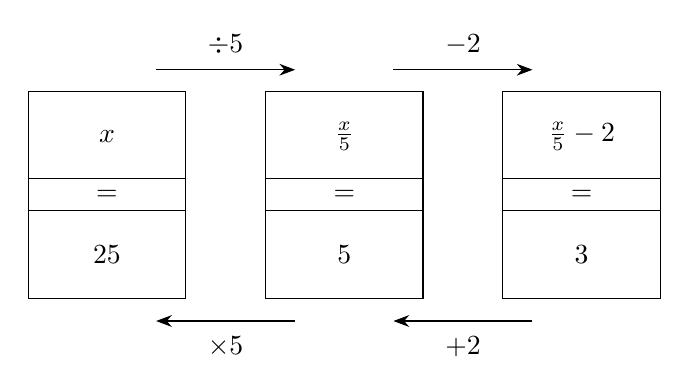
\begin{tikzpicture}[baseline={([yshift=-12pt]current bounding box.north)}]
            
        \node[backtrack] (boxA) at (0, 0) {$x$};
        \node[backtrack] (boxB) [right=1cm of boxA] {$\frac{x}{5}$};
        \node[backtrack] (boxC) [right=1cm of boxB] {$\frac{x}{5} - 2$};
    
        \node[backtrackeq] (boxAeq) [below=-1pt of boxA] {$=$};
        \node[backtrackeq] (boxBeq) [below=-1pt of boxB] {$=$};
        \node[backtrackeq] (boxCeq) [below=-1pt of boxC] {$=$};
        
        \node[backtrack] (boxArev) [below=-1pt of boxAeq] {$25$};
        \node[backtrack] (boxBrev) [below=-1pt of boxBeq] {$5$};
        \node[backtrack] (boxCrev) [below=-1pt of boxCeq] {$3$};
         
        \node (boxAr) at ([yshift=24pt,xshift=5mm]boxA) { };
        \node (boxBl) at ([yshift=24pt,xshift=-5mm]boxB) { };
        \draw [line width=0.4pt,-{Stealth[length=2mm]}] (boxAr)  --node[backtrackstep, above=3.0pt] {$\div5$} (boxBl);
    
        \node (boxBr) at ([yshift=24pt,xshift=5mm]boxB) { };
        \node (boxCl) at ([yshift=24pt,xshift=-5mm]boxC) { };
        \draw [line width=0.4pt,-{Stealth[length=2mm]}] (boxBr)  --node[backtrackstep, above=3.0pt] {$-2$} (boxCl);
    
        \node (boxCrevl) at ([yshift=-24pt,xshift=-5mm]boxCrev) { };
        \node (boxBrevr) at ([yshift=-24pt,xshift=5mm]boxBrev) { };
        \draw [line width=0.4pt,-{Stealth[length=2mm]}] (boxCrevl)  --node[backtrackstep, below=3.0pt] {$+2$} (boxBrevr);
    
        \node (boxBrevl) at ([yshift=-24pt,xshift=-5mm]boxBrev) { };
        \node (boxArevr) at ([yshift=-24pt,xshift=5mm]boxArev) { };
        \draw [line width=0.4pt,-{Stealth[length=2mm]}] (boxBrevl)  --node[backtrackstep, below=3.0pt] {$\times5$} (boxArevr);
        
    \end{tikzpicture}    
\end{equation}


\vspace{-2pt}\begin{equation}
    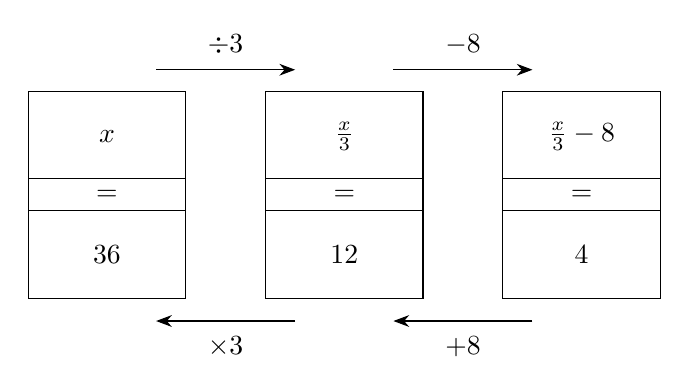
\begin{tikzpicture}[baseline={([yshift=-12pt]current bounding box.north)}]
            
        \node[backtrack] (boxA) at (0, 0) {$x$};
        \node[backtrack] (boxB) [right=1cm of boxA] {$\frac{x}{3}$};
        \node[backtrack] (boxC) [right=1cm of boxB] {$\frac{x}{3} - 8$};
    
        \node[backtrackeq] (boxAeq) [below=-1pt of boxA] {$=$};
        \node[backtrackeq] (boxBeq) [below=-1pt of boxB] {$=$};
        \node[backtrackeq] (boxCeq) [below=-1pt of boxC] {$=$};
        
        \node[backtrack] (boxArev) [below=-1pt of boxAeq] {$36$};
        \node[backtrack] (boxBrev) [below=-1pt of boxBeq] {$12$};
        \node[backtrack] (boxCrev) [below=-1pt of boxCeq] {$4$};
         
        \node (boxAr) at ([yshift=24pt,xshift=5mm]boxA) { };
        \node (boxBl) at ([yshift=24pt,xshift=-5mm]boxB) { };
        \draw [line width=0.4pt,-{Stealth[length=2mm]}] (boxAr)  --node[backtrackstep, above=3.0pt] {$\div3$} (boxBl);
    
        \node (boxBr) at ([yshift=24pt,xshift=5mm]boxB) { };
        \node (boxCl) at ([yshift=24pt,xshift=-5mm]boxC) { };
        \draw [line width=0.4pt,-{Stealth[length=2mm]}] (boxBr)  --node[backtrackstep, above=3.0pt] {$-8$} (boxCl);
    
        \node (boxCrevl) at ([yshift=-24pt,xshift=-5mm]boxCrev) { };
        \node (boxBrevr) at ([yshift=-24pt,xshift=5mm]boxBrev) { };
        \draw [line width=0.4pt,-{Stealth[length=2mm]}] (boxCrevl)  --node[backtrackstep, below=3.0pt] {$+8$} (boxBrevr);
    
        \node (boxBrevl) at ([yshift=-24pt,xshift=-5mm]boxBrev) { };
        \node (boxArevr) at ([yshift=-24pt,xshift=5mm]boxArev) { };
        \draw [line width=0.4pt,-{Stealth[length=2mm]}] (boxBrevl)  --node[backtrackstep, below=3.0pt] {$\times3$} (boxArevr);
        
    \end{tikzpicture}    
\end{equation}


\vspace{-2pt}\begin{equation}
    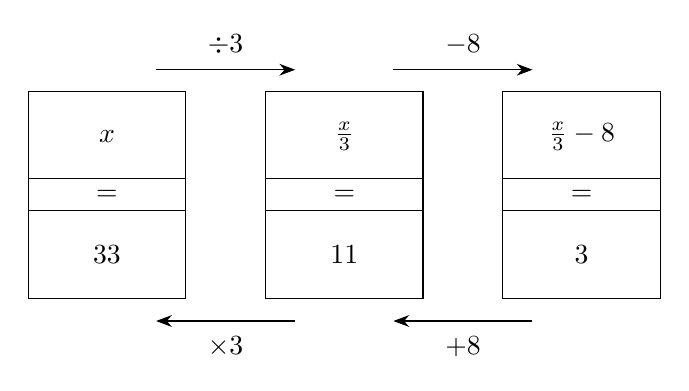
\begin{tikzpicture}[baseline={([yshift=-12pt]current bounding box.north)}]
            
        \node[backtrack] (boxA) at (0, 0) {$x$};
        \node[backtrack] (boxB) [right=1cm of boxA] {$\frac{x}{3}$};
        \node[backtrack] (boxC) [right=1cm of boxB] {$\frac{x}{3} - 8$};
    
        \node[backtrackeq] (boxAeq) [below=-1pt of boxA] {$=$};
        \node[backtrackeq] (boxBeq) [below=-1pt of boxB] {$=$};
        \node[backtrackeq] (boxCeq) [below=-1pt of boxC] {$=$};
        
        \node[backtrack] (boxArev) [below=-1pt of boxAeq] {$33$};
        \node[backtrack] (boxBrev) [below=-1pt of boxBeq] {$11$};
        \node[backtrack] (boxCrev) [below=-1pt of boxCeq] {$3$};
         
        \node (boxAr) at ([yshift=24pt,xshift=5mm]boxA) { };
        \node (boxBl) at ([yshift=24pt,xshift=-5mm]boxB) { };
        \draw [line width=0.4pt,-{Stealth[length=2mm]}] (boxAr)  --node[backtrackstep, above=3.0pt] {$\div3$} (boxBl);
    
        \node (boxBr) at ([yshift=24pt,xshift=5mm]boxB) { };
        \node (boxCl) at ([yshift=24pt,xshift=-5mm]boxC) { };
        \draw [line width=0.4pt,-{Stealth[length=2mm]}] (boxBr)  --node[backtrackstep, above=3.0pt] {$-8$} (boxCl);
    
        \node (boxCrevl) at ([yshift=-24pt,xshift=-5mm]boxCrev) { };
        \node (boxBrevr) at ([yshift=-24pt,xshift=5mm]boxBrev) { };
        \draw [line width=0.4pt,-{Stealth[length=2mm]}] (boxCrevl)  --node[backtrackstep, below=3.0pt] {$+8$} (boxBrevr);
    
        \node (boxBrevl) at ([yshift=-24pt,xshift=-5mm]boxBrev) { };
        \node (boxArevr) at ([yshift=-24pt,xshift=5mm]boxArev) { };
        \draw [line width=0.4pt,-{Stealth[length=2mm]}] (boxBrevl)  --node[backtrackstep, below=3.0pt] {$\times3$} (boxArevr);
        
    \end{tikzpicture}    
\end{equation}


\vspace{-2pt}\begin{equation}
    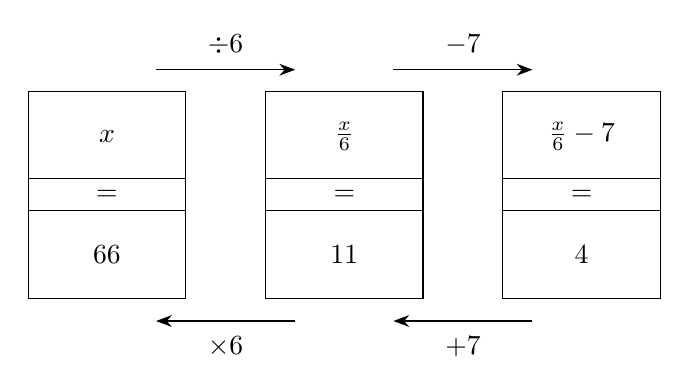
\begin{tikzpicture}[baseline={([yshift=-12pt]current bounding box.north)}]
            
        \node[backtrack] (boxA) at (0, 0) {$x$};
        \node[backtrack] (boxB) [right=1cm of boxA] {$\frac{x}{6}$};
        \node[backtrack] (boxC) [right=1cm of boxB] {$\frac{x}{6} - 7$};
    
        \node[backtrackeq] (boxAeq) [below=-1pt of boxA] {$=$};
        \node[backtrackeq] (boxBeq) [below=-1pt of boxB] {$=$};
        \node[backtrackeq] (boxCeq) [below=-1pt of boxC] {$=$};
        
        \node[backtrack] (boxArev) [below=-1pt of boxAeq] {$66$};
        \node[backtrack] (boxBrev) [below=-1pt of boxBeq] {$11$};
        \node[backtrack] (boxCrev) [below=-1pt of boxCeq] {$4$};
         
        \node (boxAr) at ([yshift=24pt,xshift=5mm]boxA) { };
        \node (boxBl) at ([yshift=24pt,xshift=-5mm]boxB) { };
        \draw [line width=0.4pt,-{Stealth[length=2mm]}] (boxAr)  --node[backtrackstep, above=3.0pt] {$\div6$} (boxBl);
    
        \node (boxBr) at ([yshift=24pt,xshift=5mm]boxB) { };
        \node (boxCl) at ([yshift=24pt,xshift=-5mm]boxC) { };
        \draw [line width=0.4pt,-{Stealth[length=2mm]}] (boxBr)  --node[backtrackstep, above=3.0pt] {$-7$} (boxCl);
    
        \node (boxCrevl) at ([yshift=-24pt,xshift=-5mm]boxCrev) { };
        \node (boxBrevr) at ([yshift=-24pt,xshift=5mm]boxBrev) { };
        \draw [line width=0.4pt,-{Stealth[length=2mm]}] (boxCrevl)  --node[backtrackstep, below=3.0pt] {$+7$} (boxBrevr);
    
        \node (boxBrevl) at ([yshift=-24pt,xshift=-5mm]boxBrev) { };
        \node (boxArevr) at ([yshift=-24pt,xshift=5mm]boxArev) { };
        \draw [line width=0.4pt,-{Stealth[length=2mm]}] (boxBrevl)  --node[backtrackstep, below=3.0pt] {$\times6$} (boxArevr);
        
    \end{tikzpicture}    
\end{equation}


\vspace{-2pt}\begin{equation}
    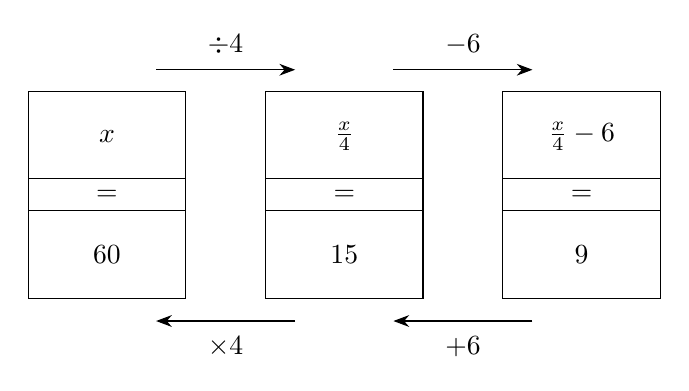
\begin{tikzpicture}[baseline={([yshift=-12pt]current bounding box.north)}]
            
        \node[backtrack] (boxA) at (0, 0) {$x$};
        \node[backtrack] (boxB) [right=1cm of boxA] {$\frac{x}{4}$};
        \node[backtrack] (boxC) [right=1cm of boxB] {$\frac{x}{4} - 6$};
    
        \node[backtrackeq] (boxAeq) [below=-1pt of boxA] {$=$};
        \node[backtrackeq] (boxBeq) [below=-1pt of boxB] {$=$};
        \node[backtrackeq] (boxCeq) [below=-1pt of boxC] {$=$};
        
        \node[backtrack] (boxArev) [below=-1pt of boxAeq] {$60$};
        \node[backtrack] (boxBrev) [below=-1pt of boxBeq] {$15$};
        \node[backtrack] (boxCrev) [below=-1pt of boxCeq] {$9$};
         
        \node (boxAr) at ([yshift=24pt,xshift=5mm]boxA) { };
        \node (boxBl) at ([yshift=24pt,xshift=-5mm]boxB) { };
        \draw [line width=0.4pt,-{Stealth[length=2mm]}] (boxAr)  --node[backtrackstep, above=3.0pt] {$\div4$} (boxBl);
    
        \node (boxBr) at ([yshift=24pt,xshift=5mm]boxB) { };
        \node (boxCl) at ([yshift=24pt,xshift=-5mm]boxC) { };
        \draw [line width=0.4pt,-{Stealth[length=2mm]}] (boxBr)  --node[backtrackstep, above=3.0pt] {$-6$} (boxCl);
    
        \node (boxCrevl) at ([yshift=-24pt,xshift=-5mm]boxCrev) { };
        \node (boxBrevr) at ([yshift=-24pt,xshift=5mm]boxBrev) { };
        \draw [line width=0.4pt,-{Stealth[length=2mm]}] (boxCrevl)  --node[backtrackstep, below=3.0pt] {$+6$} (boxBrevr);
    
        \node (boxBrevl) at ([yshift=-24pt,xshift=-5mm]boxBrev) { };
        \node (boxArevr) at ([yshift=-24pt,xshift=5mm]boxArev) { };
        \draw [line width=0.4pt,-{Stealth[length=2mm]}] (boxBrevl)  --node[backtrackstep, below=3.0pt] {$\times4$} (boxArevr);
        
    \end{tikzpicture}    
\end{equation}


\vspace{-2pt}\begin{equation}
    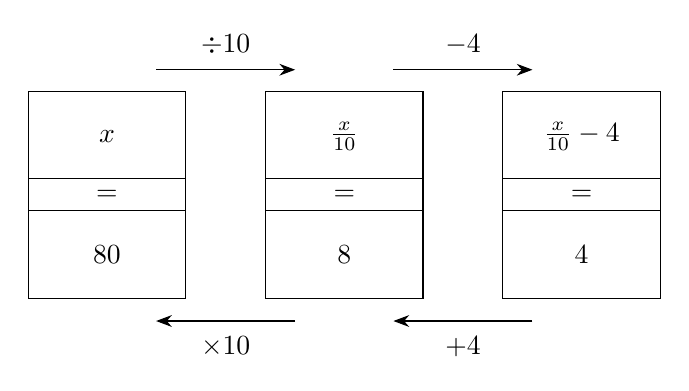
\begin{tikzpicture}[baseline={([yshift=-12pt]current bounding box.north)}]
            
        \node[backtrack] (boxA) at (0, 0) {$x$};
        \node[backtrack] (boxB) [right=1cm of boxA] {$\frac{x}{10}$};
        \node[backtrack] (boxC) [right=1cm of boxB] {$\frac{x}{10} - 4$};
    
        \node[backtrackeq] (boxAeq) [below=-1pt of boxA] {$=$};
        \node[backtrackeq] (boxBeq) [below=-1pt of boxB] {$=$};
        \node[backtrackeq] (boxCeq) [below=-1pt of boxC] {$=$};
        
        \node[backtrack] (boxArev) [below=-1pt of boxAeq] {$80$};
        \node[backtrack] (boxBrev) [below=-1pt of boxBeq] {$8$};
        \node[backtrack] (boxCrev) [below=-1pt of boxCeq] {$4$};
         
        \node (boxAr) at ([yshift=24pt,xshift=5mm]boxA) { };
        \node (boxBl) at ([yshift=24pt,xshift=-5mm]boxB) { };
        \draw [line width=0.4pt,-{Stealth[length=2mm]}] (boxAr)  --node[backtrackstep, above=3.0pt] {$\div10$} (boxBl);
    
        \node (boxBr) at ([yshift=24pt,xshift=5mm]boxB) { };
        \node (boxCl) at ([yshift=24pt,xshift=-5mm]boxC) { };
        \draw [line width=0.4pt,-{Stealth[length=2mm]}] (boxBr)  --node[backtrackstep, above=3.0pt] {$-4$} (boxCl);
    
        \node (boxCrevl) at ([yshift=-24pt,xshift=-5mm]boxCrev) { };
        \node (boxBrevr) at ([yshift=-24pt,xshift=5mm]boxBrev) { };
        \draw [line width=0.4pt,-{Stealth[length=2mm]}] (boxCrevl)  --node[backtrackstep, below=3.0pt] {$+4$} (boxBrevr);
    
        \node (boxBrevl) at ([yshift=-24pt,xshift=-5mm]boxBrev) { };
        \node (boxArevr) at ([yshift=-24pt,xshift=5mm]boxArev) { };
        \draw [line width=0.4pt,-{Stealth[length=2mm]}] (boxBrevl)  --node[backtrackstep, below=3.0pt] {$\times10$} (boxArevr);
        
    \end{tikzpicture}    
\end{equation}


\vspace{-2pt}\begin{equation}
    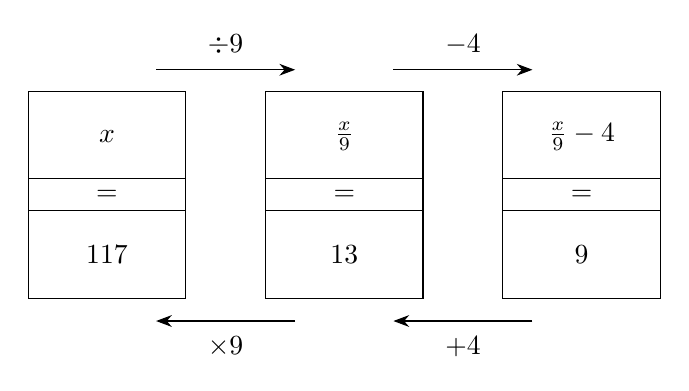
\begin{tikzpicture}[baseline={([yshift=-12pt]current bounding box.north)}]
            
        \node[backtrack] (boxA) at (0, 0) {$x$};
        \node[backtrack] (boxB) [right=1cm of boxA] {$\frac{x}{9}$};
        \node[backtrack] (boxC) [right=1cm of boxB] {$\frac{x}{9} - 4$};
    
        \node[backtrackeq] (boxAeq) [below=-1pt of boxA] {$=$};
        \node[backtrackeq] (boxBeq) [below=-1pt of boxB] {$=$};
        \node[backtrackeq] (boxCeq) [below=-1pt of boxC] {$=$};
        
        \node[backtrack] (boxArev) [below=-1pt of boxAeq] {$117$};
        \node[backtrack] (boxBrev) [below=-1pt of boxBeq] {$13$};
        \node[backtrack] (boxCrev) [below=-1pt of boxCeq] {$9$};
         
        \node (boxAr) at ([yshift=24pt,xshift=5mm]boxA) { };
        \node (boxBl) at ([yshift=24pt,xshift=-5mm]boxB) { };
        \draw [line width=0.4pt,-{Stealth[length=2mm]}] (boxAr)  --node[backtrackstep, above=3.0pt] {$\div9$} (boxBl);
    
        \node (boxBr) at ([yshift=24pt,xshift=5mm]boxB) { };
        \node (boxCl) at ([yshift=24pt,xshift=-5mm]boxC) { };
        \draw [line width=0.4pt,-{Stealth[length=2mm]}] (boxBr)  --node[backtrackstep, above=3.0pt] {$-4$} (boxCl);
    
        \node (boxCrevl) at ([yshift=-24pt,xshift=-5mm]boxCrev) { };
        \node (boxBrevr) at ([yshift=-24pt,xshift=5mm]boxBrev) { };
        \draw [line width=0.4pt,-{Stealth[length=2mm]}] (boxCrevl)  --node[backtrackstep, below=3.0pt] {$+4$} (boxBrevr);
    
        \node (boxBrevl) at ([yshift=-24pt,xshift=-5mm]boxBrev) { };
        \node (boxArevr) at ([yshift=-24pt,xshift=5mm]boxArev) { };
        \draw [line width=0.4pt,-{Stealth[length=2mm]}] (boxBrevl)  --node[backtrackstep, below=3.0pt] {$\times9$} (boxArevr);
        
    \end{tikzpicture}    
\end{equation}


\vspace{-2pt}\begin{equation}
    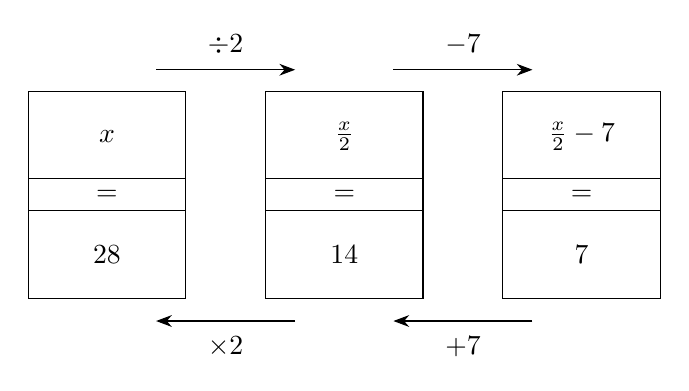
\begin{tikzpicture}[baseline={([yshift=-12pt]current bounding box.north)}]
            
        \node[backtrack] (boxA) at (0, 0) {$x$};
        \node[backtrack] (boxB) [right=1cm of boxA] {$\frac{x}{2}$};
        \node[backtrack] (boxC) [right=1cm of boxB] {$\frac{x}{2} - 7$};
    
        \node[backtrackeq] (boxAeq) [below=-1pt of boxA] {$=$};
        \node[backtrackeq] (boxBeq) [below=-1pt of boxB] {$=$};
        \node[backtrackeq] (boxCeq) [below=-1pt of boxC] {$=$};
        
        \node[backtrack] (boxArev) [below=-1pt of boxAeq] {$28$};
        \node[backtrack] (boxBrev) [below=-1pt of boxBeq] {$14$};
        \node[backtrack] (boxCrev) [below=-1pt of boxCeq] {$7$};
         
        \node (boxAr) at ([yshift=24pt,xshift=5mm]boxA) { };
        \node (boxBl) at ([yshift=24pt,xshift=-5mm]boxB) { };
        \draw [line width=0.4pt,-{Stealth[length=2mm]}] (boxAr)  --node[backtrackstep, above=3.0pt] {$\div2$} (boxBl);
    
        \node (boxBr) at ([yshift=24pt,xshift=5mm]boxB) { };
        \node (boxCl) at ([yshift=24pt,xshift=-5mm]boxC) { };
        \draw [line width=0.4pt,-{Stealth[length=2mm]}] (boxBr)  --node[backtrackstep, above=3.0pt] {$-7$} (boxCl);
    
        \node (boxCrevl) at ([yshift=-24pt,xshift=-5mm]boxCrev) { };
        \node (boxBrevr) at ([yshift=-24pt,xshift=5mm]boxBrev) { };
        \draw [line width=0.4pt,-{Stealth[length=2mm]}] (boxCrevl)  --node[backtrackstep, below=3.0pt] {$+7$} (boxBrevr);
    
        \node (boxBrevl) at ([yshift=-24pt,xshift=-5mm]boxBrev) { };
        \node (boxArevr) at ([yshift=-24pt,xshift=5mm]boxArev) { };
        \draw [line width=0.4pt,-{Stealth[length=2mm]}] (boxBrevl)  --node[backtrackstep, below=3.0pt] {$\times2$} (boxArevr);
        
    \end{tikzpicture}    
\end{equation}


\vspace{-2pt}\begin{equation}
    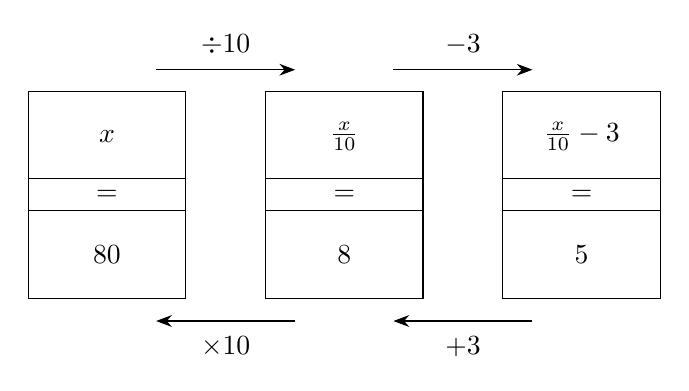
\begin{tikzpicture}[baseline={([yshift=-12pt]current bounding box.north)}]
            
        \node[backtrack] (boxA) at (0, 0) {$x$};
        \node[backtrack] (boxB) [right=1cm of boxA] {$\frac{x}{10}$};
        \node[backtrack] (boxC) [right=1cm of boxB] {$\frac{x}{10} - 3$};
    
        \node[backtrackeq] (boxAeq) [below=-1pt of boxA] {$=$};
        \node[backtrackeq] (boxBeq) [below=-1pt of boxB] {$=$};
        \node[backtrackeq] (boxCeq) [below=-1pt of boxC] {$=$};
        
        \node[backtrack] (boxArev) [below=-1pt of boxAeq] {$80$};
        \node[backtrack] (boxBrev) [below=-1pt of boxBeq] {$8$};
        \node[backtrack] (boxCrev) [below=-1pt of boxCeq] {$5$};
         
        \node (boxAr) at ([yshift=24pt,xshift=5mm]boxA) { };
        \node (boxBl) at ([yshift=24pt,xshift=-5mm]boxB) { };
        \draw [line width=0.4pt,-{Stealth[length=2mm]}] (boxAr)  --node[backtrackstep, above=3.0pt] {$\div10$} (boxBl);
    
        \node (boxBr) at ([yshift=24pt,xshift=5mm]boxB) { };
        \node (boxCl) at ([yshift=24pt,xshift=-5mm]boxC) { };
        \draw [line width=0.4pt,-{Stealth[length=2mm]}] (boxBr)  --node[backtrackstep, above=3.0pt] {$-3$} (boxCl);
    
        \node (boxCrevl) at ([yshift=-24pt,xshift=-5mm]boxCrev) { };
        \node (boxBrevr) at ([yshift=-24pt,xshift=5mm]boxBrev) { };
        \draw [line width=0.4pt,-{Stealth[length=2mm]}] (boxCrevl)  --node[backtrackstep, below=3.0pt] {$+3$} (boxBrevr);
    
        \node (boxBrevl) at ([yshift=-24pt,xshift=-5mm]boxBrev) { };
        \node (boxArevr) at ([yshift=-24pt,xshift=5mm]boxArev) { };
        \draw [line width=0.4pt,-{Stealth[length=2mm]}] (boxBrevl)  --node[backtrackstep, below=3.0pt] {$\times10$} (boxArevr);
        
    \end{tikzpicture}    
\end{equation}


\vspace{-2pt}\begin{equation}
    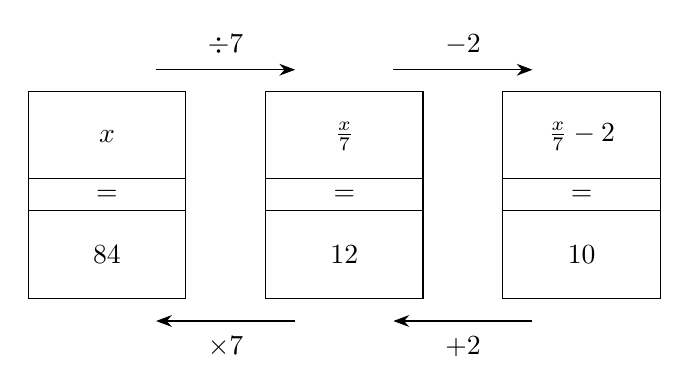
\begin{tikzpicture}[baseline={([yshift=-12pt]current bounding box.north)}]
            
        \node[backtrack] (boxA) at (0, 0) {$x$};
        \node[backtrack] (boxB) [right=1cm of boxA] {$\frac{x}{7}$};
        \node[backtrack] (boxC) [right=1cm of boxB] {$\frac{x}{7} - 2$};
    
        \node[backtrackeq] (boxAeq) [below=-1pt of boxA] {$=$};
        \node[backtrackeq] (boxBeq) [below=-1pt of boxB] {$=$};
        \node[backtrackeq] (boxCeq) [below=-1pt of boxC] {$=$};
        
        \node[backtrack] (boxArev) [below=-1pt of boxAeq] {$84$};
        \node[backtrack] (boxBrev) [below=-1pt of boxBeq] {$12$};
        \node[backtrack] (boxCrev) [below=-1pt of boxCeq] {$10$};
         
        \node (boxAr) at ([yshift=24pt,xshift=5mm]boxA) { };
        \node (boxBl) at ([yshift=24pt,xshift=-5mm]boxB) { };
        \draw [line width=0.4pt,-{Stealth[length=2mm]}] (boxAr)  --node[backtrackstep, above=3.0pt] {$\div7$} (boxBl);
    
        \node (boxBr) at ([yshift=24pt,xshift=5mm]boxB) { };
        \node (boxCl) at ([yshift=24pt,xshift=-5mm]boxC) { };
        \draw [line width=0.4pt,-{Stealth[length=2mm]}] (boxBr)  --node[backtrackstep, above=3.0pt] {$-2$} (boxCl);
    
        \node (boxCrevl) at ([yshift=-24pt,xshift=-5mm]boxCrev) { };
        \node (boxBrevr) at ([yshift=-24pt,xshift=5mm]boxBrev) { };
        \draw [line width=0.4pt,-{Stealth[length=2mm]}] (boxCrevl)  --node[backtrackstep, below=3.0pt] {$+2$} (boxBrevr);
    
        \node (boxBrevl) at ([yshift=-24pt,xshift=-5mm]boxBrev) { };
        \node (boxArevr) at ([yshift=-24pt,xshift=5mm]boxArev) { };
        \draw [line width=0.4pt,-{Stealth[length=2mm]}] (boxBrevl)  --node[backtrackstep, below=3.0pt] {$\times7$} (boxArevr);
        
    \end{tikzpicture}    
\end{equation}


\vspace{-2pt}\begin{equation}
    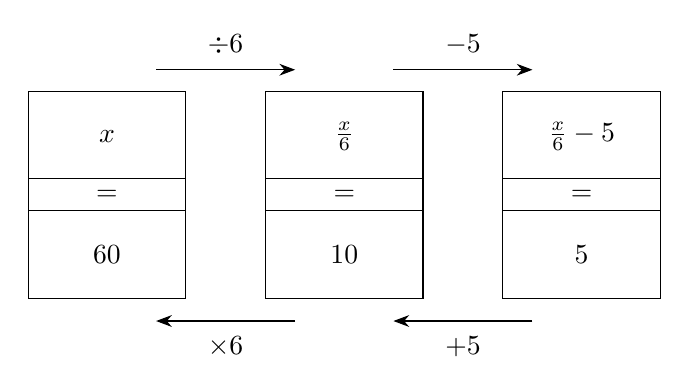
\begin{tikzpicture}[baseline={([yshift=-12pt]current bounding box.north)}]
            
        \node[backtrack] (boxA) at (0, 0) {$x$};
        \node[backtrack] (boxB) [right=1cm of boxA] {$\frac{x}{6}$};
        \node[backtrack] (boxC) [right=1cm of boxB] {$\frac{x}{6} - 5$};
    
        \node[backtrackeq] (boxAeq) [below=-1pt of boxA] {$=$};
        \node[backtrackeq] (boxBeq) [below=-1pt of boxB] {$=$};
        \node[backtrackeq] (boxCeq) [below=-1pt of boxC] {$=$};
        
        \node[backtrack] (boxArev) [below=-1pt of boxAeq] {$60$};
        \node[backtrack] (boxBrev) [below=-1pt of boxBeq] {$10$};
        \node[backtrack] (boxCrev) [below=-1pt of boxCeq] {$5$};
         
        \node (boxAr) at ([yshift=24pt,xshift=5mm]boxA) { };
        \node (boxBl) at ([yshift=24pt,xshift=-5mm]boxB) { };
        \draw [line width=0.4pt,-{Stealth[length=2mm]}] (boxAr)  --node[backtrackstep, above=3.0pt] {$\div6$} (boxBl);
    
        \node (boxBr) at ([yshift=24pt,xshift=5mm]boxB) { };
        \node (boxCl) at ([yshift=24pt,xshift=-5mm]boxC) { };
        \draw [line width=0.4pt,-{Stealth[length=2mm]}] (boxBr)  --node[backtrackstep, above=3.0pt] {$-5$} (boxCl);
    
        \node (boxCrevl) at ([yshift=-24pt,xshift=-5mm]boxCrev) { };
        \node (boxBrevr) at ([yshift=-24pt,xshift=5mm]boxBrev) { };
        \draw [line width=0.4pt,-{Stealth[length=2mm]}] (boxCrevl)  --node[backtrackstep, below=3.0pt] {$+5$} (boxBrevr);
    
        \node (boxBrevl) at ([yshift=-24pt,xshift=-5mm]boxBrev) { };
        \node (boxArevr) at ([yshift=-24pt,xshift=5mm]boxArev) { };
        \draw [line width=0.4pt,-{Stealth[length=2mm]}] (boxBrevl)  --node[backtrackstep, below=3.0pt] {$\times6$} (boxArevr);
        
    \end{tikzpicture}    
\end{equation}


\vspace{-2pt}\begin{equation}
    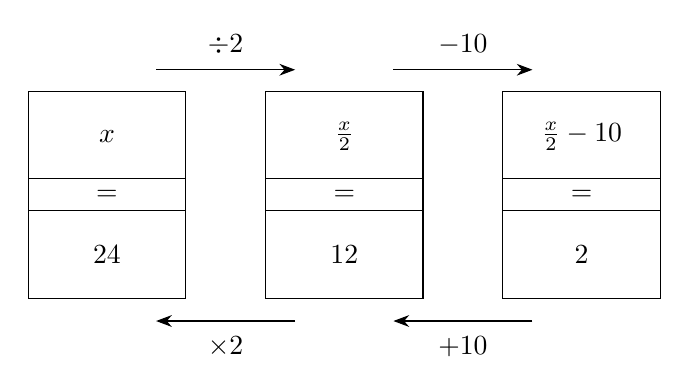
\begin{tikzpicture}[baseline={([yshift=-12pt]current bounding box.north)}]
            
        \node[backtrack] (boxA) at (0, 0) {$x$};
        \node[backtrack] (boxB) [right=1cm of boxA] {$\frac{x}{2}$};
        \node[backtrack] (boxC) [right=1cm of boxB] {$\frac{x}{2} - 10$};
    
        \node[backtrackeq] (boxAeq) [below=-1pt of boxA] {$=$};
        \node[backtrackeq] (boxBeq) [below=-1pt of boxB] {$=$};
        \node[backtrackeq] (boxCeq) [below=-1pt of boxC] {$=$};
        
        \node[backtrack] (boxArev) [below=-1pt of boxAeq] {$24$};
        \node[backtrack] (boxBrev) [below=-1pt of boxBeq] {$12$};
        \node[backtrack] (boxCrev) [below=-1pt of boxCeq] {$2$};
         
        \node (boxAr) at ([yshift=24pt,xshift=5mm]boxA) { };
        \node (boxBl) at ([yshift=24pt,xshift=-5mm]boxB) { };
        \draw [line width=0.4pt,-{Stealth[length=2mm]}] (boxAr)  --node[backtrackstep, above=3.0pt] {$\div2$} (boxBl);
    
        \node (boxBr) at ([yshift=24pt,xshift=5mm]boxB) { };
        \node (boxCl) at ([yshift=24pt,xshift=-5mm]boxC) { };
        \draw [line width=0.4pt,-{Stealth[length=2mm]}] (boxBr)  --node[backtrackstep, above=3.0pt] {$-10$} (boxCl);
    
        \node (boxCrevl) at ([yshift=-24pt,xshift=-5mm]boxCrev) { };
        \node (boxBrevr) at ([yshift=-24pt,xshift=5mm]boxBrev) { };
        \draw [line width=0.4pt,-{Stealth[length=2mm]}] (boxCrevl)  --node[backtrackstep, below=3.0pt] {$+10$} (boxBrevr);
    
        \node (boxBrevl) at ([yshift=-24pt,xshift=-5mm]boxBrev) { };
        \node (boxArevr) at ([yshift=-24pt,xshift=5mm]boxArev) { };
        \draw [line width=0.4pt,-{Stealth[length=2mm]}] (boxBrevl)  --node[backtrackstep, below=3.0pt] {$\times2$} (boxArevr);
        
    \end{tikzpicture}    
\end{equation}


\vspace{-2pt}\begin{equation}
    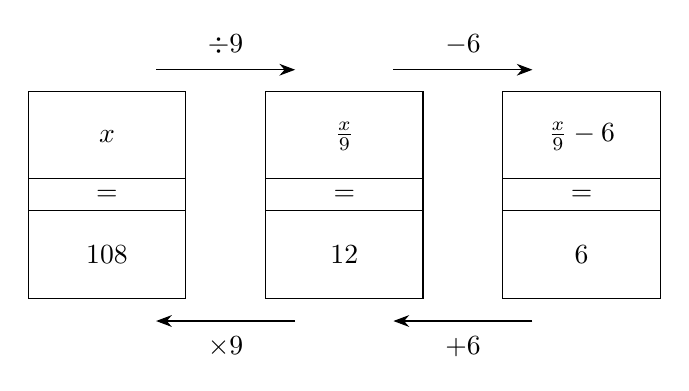
\begin{tikzpicture}[baseline={([yshift=-12pt]current bounding box.north)}]
            
        \node[backtrack] (boxA) at (0, 0) {$x$};
        \node[backtrack] (boxB) [right=1cm of boxA] {$\frac{x}{9}$};
        \node[backtrack] (boxC) [right=1cm of boxB] {$\frac{x}{9} - 6$};
    
        \node[backtrackeq] (boxAeq) [below=-1pt of boxA] {$=$};
        \node[backtrackeq] (boxBeq) [below=-1pt of boxB] {$=$};
        \node[backtrackeq] (boxCeq) [below=-1pt of boxC] {$=$};
        
        \node[backtrack] (boxArev) [below=-1pt of boxAeq] {$108$};
        \node[backtrack] (boxBrev) [below=-1pt of boxBeq] {$12$};
        \node[backtrack] (boxCrev) [below=-1pt of boxCeq] {$6$};
         
        \node (boxAr) at ([yshift=24pt,xshift=5mm]boxA) { };
        \node (boxBl) at ([yshift=24pt,xshift=-5mm]boxB) { };
        \draw [line width=0.4pt,-{Stealth[length=2mm]}] (boxAr)  --node[backtrackstep, above=3.0pt] {$\div9$} (boxBl);
    
        \node (boxBr) at ([yshift=24pt,xshift=5mm]boxB) { };
        \node (boxCl) at ([yshift=24pt,xshift=-5mm]boxC) { };
        \draw [line width=0.4pt,-{Stealth[length=2mm]}] (boxBr)  --node[backtrackstep, above=3.0pt] {$-6$} (boxCl);
    
        \node (boxCrevl) at ([yshift=-24pt,xshift=-5mm]boxCrev) { };
        \node (boxBrevr) at ([yshift=-24pt,xshift=5mm]boxBrev) { };
        \draw [line width=0.4pt,-{Stealth[length=2mm]}] (boxCrevl)  --node[backtrackstep, below=3.0pt] {$+6$} (boxBrevr);
    
        \node (boxBrevl) at ([yshift=-24pt,xshift=-5mm]boxBrev) { };
        \node (boxArevr) at ([yshift=-24pt,xshift=5mm]boxArev) { };
        \draw [line width=0.4pt,-{Stealth[length=2mm]}] (boxBrevl)  --node[backtrackstep, below=3.0pt] {$\times9$} (boxArevr);
        
    \end{tikzpicture}    
\end{equation}


\vspace{-2pt}\begin{equation}
    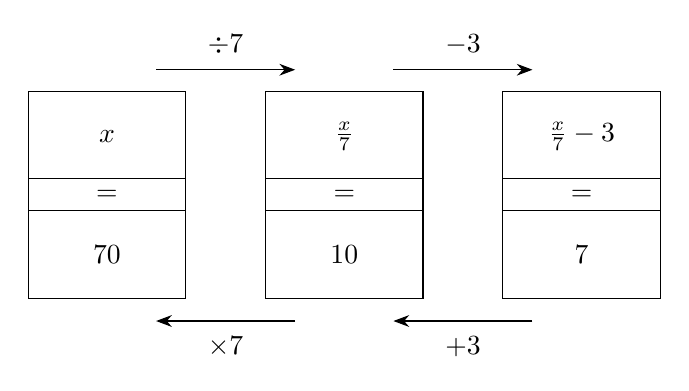
\begin{tikzpicture}[baseline={([yshift=-12pt]current bounding box.north)}]
            
        \node[backtrack] (boxA) at (0, 0) {$x$};
        \node[backtrack] (boxB) [right=1cm of boxA] {$\frac{x}{7}$};
        \node[backtrack] (boxC) [right=1cm of boxB] {$\frac{x}{7} - 3$};
    
        \node[backtrackeq] (boxAeq) [below=-1pt of boxA] {$=$};
        \node[backtrackeq] (boxBeq) [below=-1pt of boxB] {$=$};
        \node[backtrackeq] (boxCeq) [below=-1pt of boxC] {$=$};
        
        \node[backtrack] (boxArev) [below=-1pt of boxAeq] {$70$};
        \node[backtrack] (boxBrev) [below=-1pt of boxBeq] {$10$};
        \node[backtrack] (boxCrev) [below=-1pt of boxCeq] {$7$};
         
        \node (boxAr) at ([yshift=24pt,xshift=5mm]boxA) { };
        \node (boxBl) at ([yshift=24pt,xshift=-5mm]boxB) { };
        \draw [line width=0.4pt,-{Stealth[length=2mm]}] (boxAr)  --node[backtrackstep, above=3.0pt] {$\div7$} (boxBl);
    
        \node (boxBr) at ([yshift=24pt,xshift=5mm]boxB) { };
        \node (boxCl) at ([yshift=24pt,xshift=-5mm]boxC) { };
        \draw [line width=0.4pt,-{Stealth[length=2mm]}] (boxBr)  --node[backtrackstep, above=3.0pt] {$-3$} (boxCl);
    
        \node (boxCrevl) at ([yshift=-24pt,xshift=-5mm]boxCrev) { };
        \node (boxBrevr) at ([yshift=-24pt,xshift=5mm]boxBrev) { };
        \draw [line width=0.4pt,-{Stealth[length=2mm]}] (boxCrevl)  --node[backtrackstep, below=3.0pt] {$+3$} (boxBrevr);
    
        \node (boxBrevl) at ([yshift=-24pt,xshift=-5mm]boxBrev) { };
        \node (boxArevr) at ([yshift=-24pt,xshift=5mm]boxArev) { };
        \draw [line width=0.4pt,-{Stealth[length=2mm]}] (boxBrevl)  --node[backtrackstep, below=3.0pt] {$\times7$} (boxArevr);
        
    \end{tikzpicture}    
\end{equation}


\vspace{-2pt}\begin{equation}
    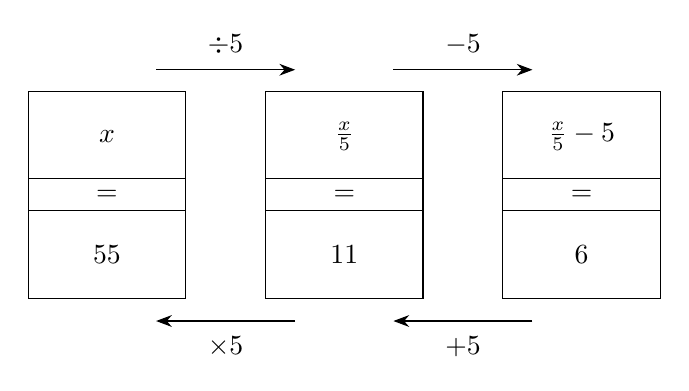
\begin{tikzpicture}[baseline={([yshift=-12pt]current bounding box.north)}]
            
        \node[backtrack] (boxA) at (0, 0) {$x$};
        \node[backtrack] (boxB) [right=1cm of boxA] {$\frac{x}{5}$};
        \node[backtrack] (boxC) [right=1cm of boxB] {$\frac{x}{5} - 5$};
    
        \node[backtrackeq] (boxAeq) [below=-1pt of boxA] {$=$};
        \node[backtrackeq] (boxBeq) [below=-1pt of boxB] {$=$};
        \node[backtrackeq] (boxCeq) [below=-1pt of boxC] {$=$};
        
        \node[backtrack] (boxArev) [below=-1pt of boxAeq] {$55$};
        \node[backtrack] (boxBrev) [below=-1pt of boxBeq] {$11$};
        \node[backtrack] (boxCrev) [below=-1pt of boxCeq] {$6$};
         
        \node (boxAr) at ([yshift=24pt,xshift=5mm]boxA) { };
        \node (boxBl) at ([yshift=24pt,xshift=-5mm]boxB) { };
        \draw [line width=0.4pt,-{Stealth[length=2mm]}] (boxAr)  --node[backtrackstep, above=3.0pt] {$\div5$} (boxBl);
    
        \node (boxBr) at ([yshift=24pt,xshift=5mm]boxB) { };
        \node (boxCl) at ([yshift=24pt,xshift=-5mm]boxC) { };
        \draw [line width=0.4pt,-{Stealth[length=2mm]}] (boxBr)  --node[backtrackstep, above=3.0pt] {$-5$} (boxCl);
    
        \node (boxCrevl) at ([yshift=-24pt,xshift=-5mm]boxCrev) { };
        \node (boxBrevr) at ([yshift=-24pt,xshift=5mm]boxBrev) { };
        \draw [line width=0.4pt,-{Stealth[length=2mm]}] (boxCrevl)  --node[backtrackstep, below=3.0pt] {$+5$} (boxBrevr);
    
        \node (boxBrevl) at ([yshift=-24pt,xshift=-5mm]boxBrev) { };
        \node (boxArevr) at ([yshift=-24pt,xshift=5mm]boxArev) { };
        \draw [line width=0.4pt,-{Stealth[length=2mm]}] (boxBrevl)  --node[backtrackstep, below=3.0pt] {$\times5$} (boxArevr);
        
    \end{tikzpicture}    
\end{equation}


\vspace{-2pt}\begin{equation}
    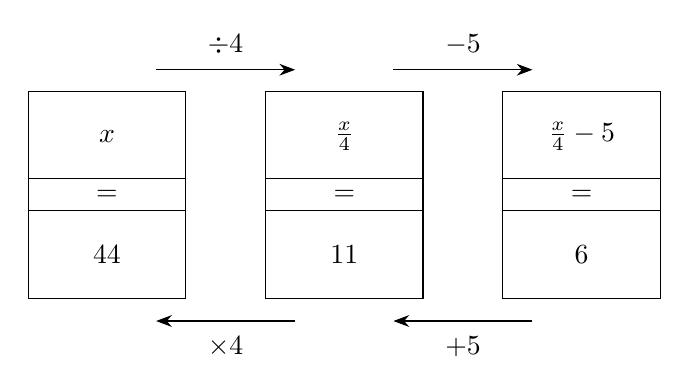
\begin{tikzpicture}[baseline={([yshift=-12pt]current bounding box.north)}]
            
        \node[backtrack] (boxA) at (0, 0) {$x$};
        \node[backtrack] (boxB) [right=1cm of boxA] {$\frac{x}{4}$};
        \node[backtrack] (boxC) [right=1cm of boxB] {$\frac{x}{4} - 5$};
    
        \node[backtrackeq] (boxAeq) [below=-1pt of boxA] {$=$};
        \node[backtrackeq] (boxBeq) [below=-1pt of boxB] {$=$};
        \node[backtrackeq] (boxCeq) [below=-1pt of boxC] {$=$};
        
        \node[backtrack] (boxArev) [below=-1pt of boxAeq] {$44$};
        \node[backtrack] (boxBrev) [below=-1pt of boxBeq] {$11$};
        \node[backtrack] (boxCrev) [below=-1pt of boxCeq] {$6$};
         
        \node (boxAr) at ([yshift=24pt,xshift=5mm]boxA) { };
        \node (boxBl) at ([yshift=24pt,xshift=-5mm]boxB) { };
        \draw [line width=0.4pt,-{Stealth[length=2mm]}] (boxAr)  --node[backtrackstep, above=3.0pt] {$\div4$} (boxBl);
    
        \node (boxBr) at ([yshift=24pt,xshift=5mm]boxB) { };
        \node (boxCl) at ([yshift=24pt,xshift=-5mm]boxC) { };
        \draw [line width=0.4pt,-{Stealth[length=2mm]}] (boxBr)  --node[backtrackstep, above=3.0pt] {$-5$} (boxCl);
    
        \node (boxCrevl) at ([yshift=-24pt,xshift=-5mm]boxCrev) { };
        \node (boxBrevr) at ([yshift=-24pt,xshift=5mm]boxBrev) { };
        \draw [line width=0.4pt,-{Stealth[length=2mm]}] (boxCrevl)  --node[backtrackstep, below=3.0pt] {$+5$} (boxBrevr);
    
        \node (boxBrevl) at ([yshift=-24pt,xshift=-5mm]boxBrev) { };
        \node (boxArevr) at ([yshift=-24pt,xshift=5mm]boxArev) { };
        \draw [line width=0.4pt,-{Stealth[length=2mm]}] (boxBrevl)  --node[backtrackstep, below=3.0pt] {$\times4$} (boxArevr);
        
    \end{tikzpicture}    
\end{equation}


\vspace{-2pt}\begin{equation}
    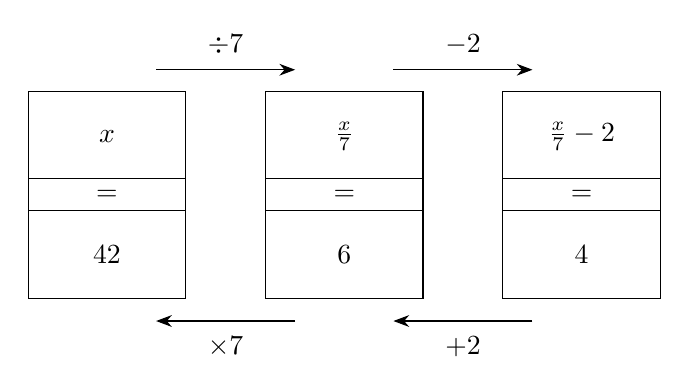
\begin{tikzpicture}[baseline={([yshift=-12pt]current bounding box.north)}]
            
        \node[backtrack] (boxA) at (0, 0) {$x$};
        \node[backtrack] (boxB) [right=1cm of boxA] {$\frac{x}{7}$};
        \node[backtrack] (boxC) [right=1cm of boxB] {$\frac{x}{7} - 2$};
    
        \node[backtrackeq] (boxAeq) [below=-1pt of boxA] {$=$};
        \node[backtrackeq] (boxBeq) [below=-1pt of boxB] {$=$};
        \node[backtrackeq] (boxCeq) [below=-1pt of boxC] {$=$};
        
        \node[backtrack] (boxArev) [below=-1pt of boxAeq] {$42$};
        \node[backtrack] (boxBrev) [below=-1pt of boxBeq] {$6$};
        \node[backtrack] (boxCrev) [below=-1pt of boxCeq] {$4$};
         
        \node (boxAr) at ([yshift=24pt,xshift=5mm]boxA) { };
        \node (boxBl) at ([yshift=24pt,xshift=-5mm]boxB) { };
        \draw [line width=0.4pt,-{Stealth[length=2mm]}] (boxAr)  --node[backtrackstep, above=3.0pt] {$\div7$} (boxBl);
    
        \node (boxBr) at ([yshift=24pt,xshift=5mm]boxB) { };
        \node (boxCl) at ([yshift=24pt,xshift=-5mm]boxC) { };
        \draw [line width=0.4pt,-{Stealth[length=2mm]}] (boxBr)  --node[backtrackstep, above=3.0pt] {$-2$} (boxCl);
    
        \node (boxCrevl) at ([yshift=-24pt,xshift=-5mm]boxCrev) { };
        \node (boxBrevr) at ([yshift=-24pt,xshift=5mm]boxBrev) { };
        \draw [line width=0.4pt,-{Stealth[length=2mm]}] (boxCrevl)  --node[backtrackstep, below=3.0pt] {$+2$} (boxBrevr);
    
        \node (boxBrevl) at ([yshift=-24pt,xshift=-5mm]boxBrev) { };
        \node (boxArevr) at ([yshift=-24pt,xshift=5mm]boxArev) { };
        \draw [line width=0.4pt,-{Stealth[length=2mm]}] (boxBrevl)  --node[backtrackstep, below=3.0pt] {$\times7$} (boxArevr);
        
    \end{tikzpicture}    
\end{equation}


\vspace{-2pt}\begin{equation}
    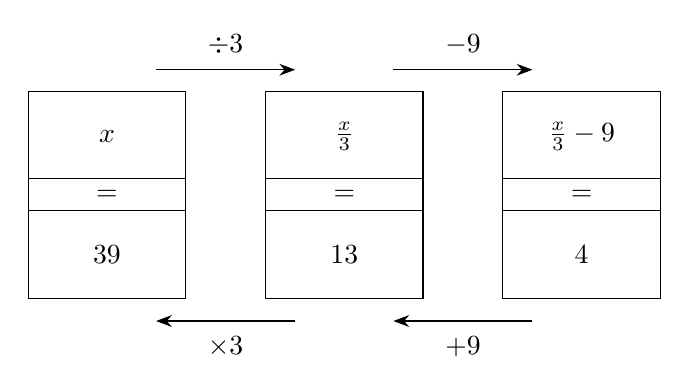
\begin{tikzpicture}[baseline={([yshift=-12pt]current bounding box.north)}]
            
        \node[backtrack] (boxA) at (0, 0) {$x$};
        \node[backtrack] (boxB) [right=1cm of boxA] {$\frac{x}{3}$};
        \node[backtrack] (boxC) [right=1cm of boxB] {$\frac{x}{3} - 9$};
    
        \node[backtrackeq] (boxAeq) [below=-1pt of boxA] {$=$};
        \node[backtrackeq] (boxBeq) [below=-1pt of boxB] {$=$};
        \node[backtrackeq] (boxCeq) [below=-1pt of boxC] {$=$};
        
        \node[backtrack] (boxArev) [below=-1pt of boxAeq] {$39$};
        \node[backtrack] (boxBrev) [below=-1pt of boxBeq] {$13$};
        \node[backtrack] (boxCrev) [below=-1pt of boxCeq] {$4$};
         
        \node (boxAr) at ([yshift=24pt,xshift=5mm]boxA) { };
        \node (boxBl) at ([yshift=24pt,xshift=-5mm]boxB) { };
        \draw [line width=0.4pt,-{Stealth[length=2mm]}] (boxAr)  --node[backtrackstep, above=3.0pt] {$\div3$} (boxBl);
    
        \node (boxBr) at ([yshift=24pt,xshift=5mm]boxB) { };
        \node (boxCl) at ([yshift=24pt,xshift=-5mm]boxC) { };
        \draw [line width=0.4pt,-{Stealth[length=2mm]}] (boxBr)  --node[backtrackstep, above=3.0pt] {$-9$} (boxCl);
    
        \node (boxCrevl) at ([yshift=-24pt,xshift=-5mm]boxCrev) { };
        \node (boxBrevr) at ([yshift=-24pt,xshift=5mm]boxBrev) { };
        \draw [line width=0.4pt,-{Stealth[length=2mm]}] (boxCrevl)  --node[backtrackstep, below=3.0pt] {$+9$} (boxBrevr);
    
        \node (boxBrevl) at ([yshift=-24pt,xshift=-5mm]boxBrev) { };
        \node (boxArevr) at ([yshift=-24pt,xshift=5mm]boxArev) { };
        \draw [line width=0.4pt,-{Stealth[length=2mm]}] (boxBrevl)  --node[backtrackstep, below=3.0pt] {$\times3$} (boxArevr);
        
    \end{tikzpicture}    
\end{equation}


\vspace{-2pt}\begin{equation}
    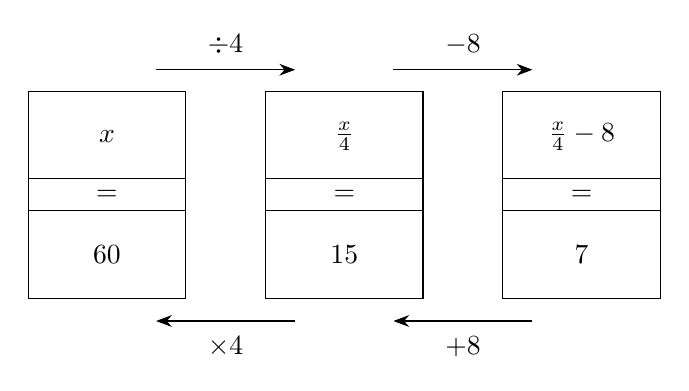
\begin{tikzpicture}[baseline={([yshift=-12pt]current bounding box.north)}]
            
        \node[backtrack] (boxA) at (0, 0) {$x$};
        \node[backtrack] (boxB) [right=1cm of boxA] {$\frac{x}{4}$};
        \node[backtrack] (boxC) [right=1cm of boxB] {$\frac{x}{4} - 8$};
    
        \node[backtrackeq] (boxAeq) [below=-1pt of boxA] {$=$};
        \node[backtrackeq] (boxBeq) [below=-1pt of boxB] {$=$};
        \node[backtrackeq] (boxCeq) [below=-1pt of boxC] {$=$};
        
        \node[backtrack] (boxArev) [below=-1pt of boxAeq] {$60$};
        \node[backtrack] (boxBrev) [below=-1pt of boxBeq] {$15$};
        \node[backtrack] (boxCrev) [below=-1pt of boxCeq] {$7$};
         
        \node (boxAr) at ([yshift=24pt,xshift=5mm]boxA) { };
        \node (boxBl) at ([yshift=24pt,xshift=-5mm]boxB) { };
        \draw [line width=0.4pt,-{Stealth[length=2mm]}] (boxAr)  --node[backtrackstep, above=3.0pt] {$\div4$} (boxBl);
    
        \node (boxBr) at ([yshift=24pt,xshift=5mm]boxB) { };
        \node (boxCl) at ([yshift=24pt,xshift=-5mm]boxC) { };
        \draw [line width=0.4pt,-{Stealth[length=2mm]}] (boxBr)  --node[backtrackstep, above=3.0pt] {$-8$} (boxCl);
    
        \node (boxCrevl) at ([yshift=-24pt,xshift=-5mm]boxCrev) { };
        \node (boxBrevr) at ([yshift=-24pt,xshift=5mm]boxBrev) { };
        \draw [line width=0.4pt,-{Stealth[length=2mm]}] (boxCrevl)  --node[backtrackstep, below=3.0pt] {$+8$} (boxBrevr);
    
        \node (boxBrevl) at ([yshift=-24pt,xshift=-5mm]boxBrev) { };
        \node (boxArevr) at ([yshift=-24pt,xshift=5mm]boxArev) { };
        \draw [line width=0.4pt,-{Stealth[length=2mm]}] (boxBrevl)  --node[backtrackstep, below=3.0pt] {$\times4$} (boxArevr);
        
    \end{tikzpicture}    
\end{equation}


\vspace{-2pt}\begin{equation}
    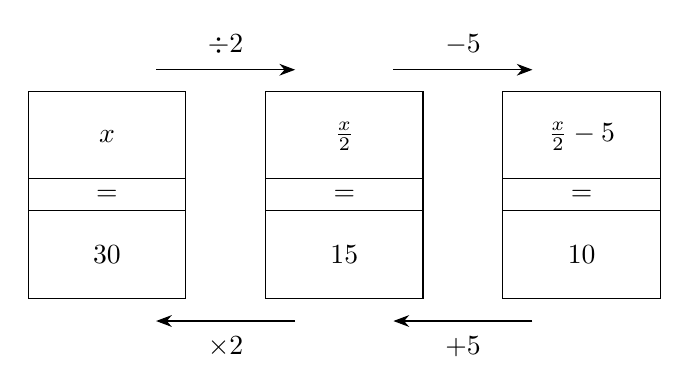
\begin{tikzpicture}[baseline={([yshift=-12pt]current bounding box.north)}]
            
        \node[backtrack] (boxA) at (0, 0) {$x$};
        \node[backtrack] (boxB) [right=1cm of boxA] {$\frac{x}{2}$};
        \node[backtrack] (boxC) [right=1cm of boxB] {$\frac{x}{2} - 5$};
    
        \node[backtrackeq] (boxAeq) [below=-1pt of boxA] {$=$};
        \node[backtrackeq] (boxBeq) [below=-1pt of boxB] {$=$};
        \node[backtrackeq] (boxCeq) [below=-1pt of boxC] {$=$};
        
        \node[backtrack] (boxArev) [below=-1pt of boxAeq] {$30$};
        \node[backtrack] (boxBrev) [below=-1pt of boxBeq] {$15$};
        \node[backtrack] (boxCrev) [below=-1pt of boxCeq] {$10$};
         
        \node (boxAr) at ([yshift=24pt,xshift=5mm]boxA) { };
        \node (boxBl) at ([yshift=24pt,xshift=-5mm]boxB) { };
        \draw [line width=0.4pt,-{Stealth[length=2mm]}] (boxAr)  --node[backtrackstep, above=3.0pt] {$\div2$} (boxBl);
    
        \node (boxBr) at ([yshift=24pt,xshift=5mm]boxB) { };
        \node (boxCl) at ([yshift=24pt,xshift=-5mm]boxC) { };
        \draw [line width=0.4pt,-{Stealth[length=2mm]}] (boxBr)  --node[backtrackstep, above=3.0pt] {$-5$} (boxCl);
    
        \node (boxCrevl) at ([yshift=-24pt,xshift=-5mm]boxCrev) { };
        \node (boxBrevr) at ([yshift=-24pt,xshift=5mm]boxBrev) { };
        \draw [line width=0.4pt,-{Stealth[length=2mm]}] (boxCrevl)  --node[backtrackstep, below=3.0pt] {$+5$} (boxBrevr);
    
        \node (boxBrevl) at ([yshift=-24pt,xshift=-5mm]boxBrev) { };
        \node (boxArevr) at ([yshift=-24pt,xshift=5mm]boxArev) { };
        \draw [line width=0.4pt,-{Stealth[length=2mm]}] (boxBrevl)  --node[backtrackstep, below=3.0pt] {$\times2$} (boxArevr);
        
    \end{tikzpicture}    
\end{equation}


\vspace{-2pt}
    \end{multicols}
\end{document}
